\documentclass[10pt, t]{beamer}
% \usepackage[UTF8]{ctex}
\usepackage{amsmath}
\usepackage{setspace}
\usepackage{float} 
\usepackage{multido}
\usepackage{multirow}
\usepackage{array}
\usepackage{enumerate}
\usepackage{booktabs}
\usepackage{indentfirst} 
\usepackage[style=mla]{biblatex}
\usepackage{setspace}
\usepackage{subcaption}
\usepackage{hyperref}
\usepackage{textpos}
% \usepackage{fontspec}

% \beamerdefaultoverlayspecification{<+->}
\makeatletter
\let\@@magyar@captionfix\relax
\makeatother

\definecolor{bladerunnerblue}{RGB}{41, 159, 163}
\definecolor{bladerunnerred}{RGB}{194,84,97}
\definecolor{themecolor}{RGB}{25,25,112} 
\definecolor{weak}{RGB}{150,150,150}

\renewcommand{\emph}[1]{{\color{themecolor}\textsl{#1}}}
\newcommand{\alarm}[1]{{\color{bladerunnerred}{#1}}}
\newcommand{\N}{\mathbb{N}}
\newcommand{\R}{\mathbb{R}}
\newcommand{\dom}{\operatorname{dom}}
\newcommand{\myseries}[2]{$#1_1,#1_2,\dots,#1_#2$}
\newcommand{\nullspace}{~\\[15pt]}
\newcommand{\remark}{\textbf{Remark: }}
\newcommand{\question}{\textbf{Question: }}
\newcommand{\scp}[2]{\langle\,#1\,,\,#2\,\rangle} \newcommand{\scpp}{\langle\,\cdot\,,\,\cdot\,\rangle}
\newcommand{\weaken}[1]{{\color{weak}\textit{#1}}}
\newcommand{\underover}[3]{\underset{#2}{\overset{#3}{#1}}}
\renewcommand{\emptyset}{\varnothing}


\usetheme{Madrid}
\setbeamertemplate{navigation symbols}{}

\addtobeamertemplate{frametitle}{}{
\begin{textblock*}{100mm}(0.85\textwidth,-1cm)
\includegraphics[height=1cm]{../../logo.png}
\end{textblock*}}


\usecolortheme[named=themecolor]{structure}

\setbeamertemplate{items}[default]

\hypersetup{
    colorlinks=true,
    linkcolor=themecolor,
    filecolor=themecolor,      
    urlcolor=themecolor,
    citecolor=themecolor,
}

\title{VV186: Honors Mathematics}
\subtitle{Series}
\institute[UM-SJTU JI]{Univerity of Michigan-Shanghai Jiao Tong University Joint Institute}
\author{Xingjian Zhang}

\begin{document}

\begin{frame}
    \titlepage
    \begin{center}
        \includegraphics[height=2cm]{../../logo2.png}
    \end{center}
\end{frame}

\begin{frame}
    \frametitle{RC Policy}
    Several things I want you to pay attention to:
    \begin{enumerate}
        \item \alarm{Be interactive.} Feel free to interrupt me at any time if you want to ask something or simply make some comments. You are free to discuss with your friend if you want, as long as your discussion is related to the course contents and your voice won't effect other students.
        \item Speak everything in \alarm{English} during the RC. This might be hard at the beginning, but you will soon get used to that.
        \item \alarm{``Question everything.''} Do not pretend to have understood everything. Maths is about strictness, abstraction and generalization. Understanding every basic concept is essential in our course. I will be quite ``push'' on checking your conceptual understanding. This process will be \textbf{annoying, tedious, but rewarding}. So Get prepared.
    \end{enumerate}
\end{frame}

\begin{frame}
    \frametitle{Outline}
    \begin{spacing}{1}
        \tableofcontents
    \end{spacing}
\end{frame}

\section{Sequence of Real Functions}
\subsection{Sequence in Vector Space}
\begin{frame}
    \frametitle{Sequences in Vector Space}
    Recall how we define convergent sequence in a metric space. Since that every normed vector space is also a metric space, we can then define convergent sequence in it.
    \begin{figure}[H]
        \centering
        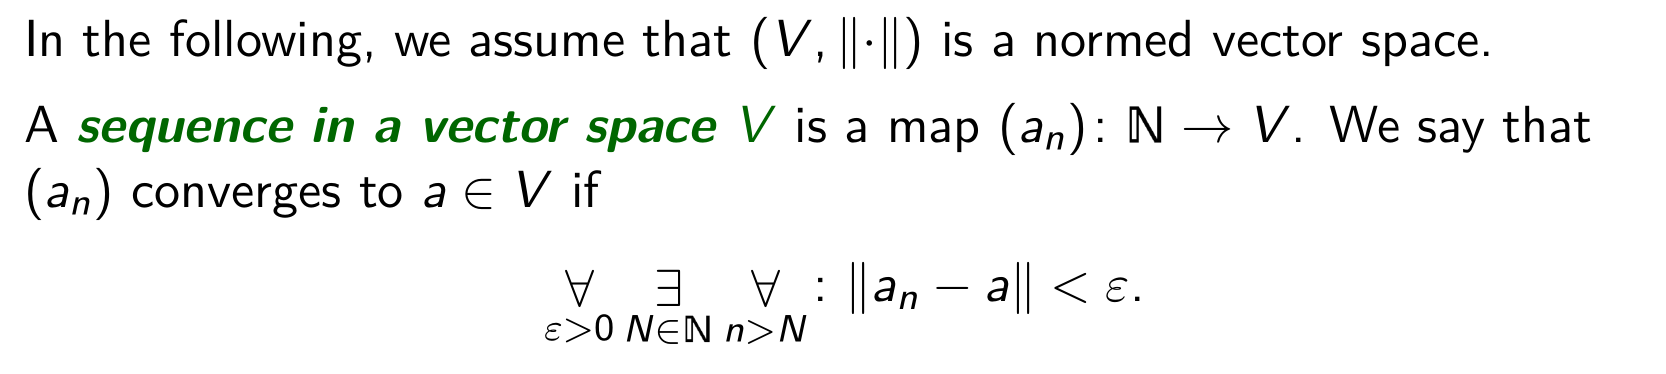
\includegraphics[width=0.9\textwidth]{2020-11-11-12-36-36.png}
    \end{figure}
\end{frame}
\subsection{Sequence of Functions}
\begin{frame}
    \frametitle{Sequence of Functions}
    We now consider two kinds of convergence for functions.
    \begin{figure}[H]
        \centering
        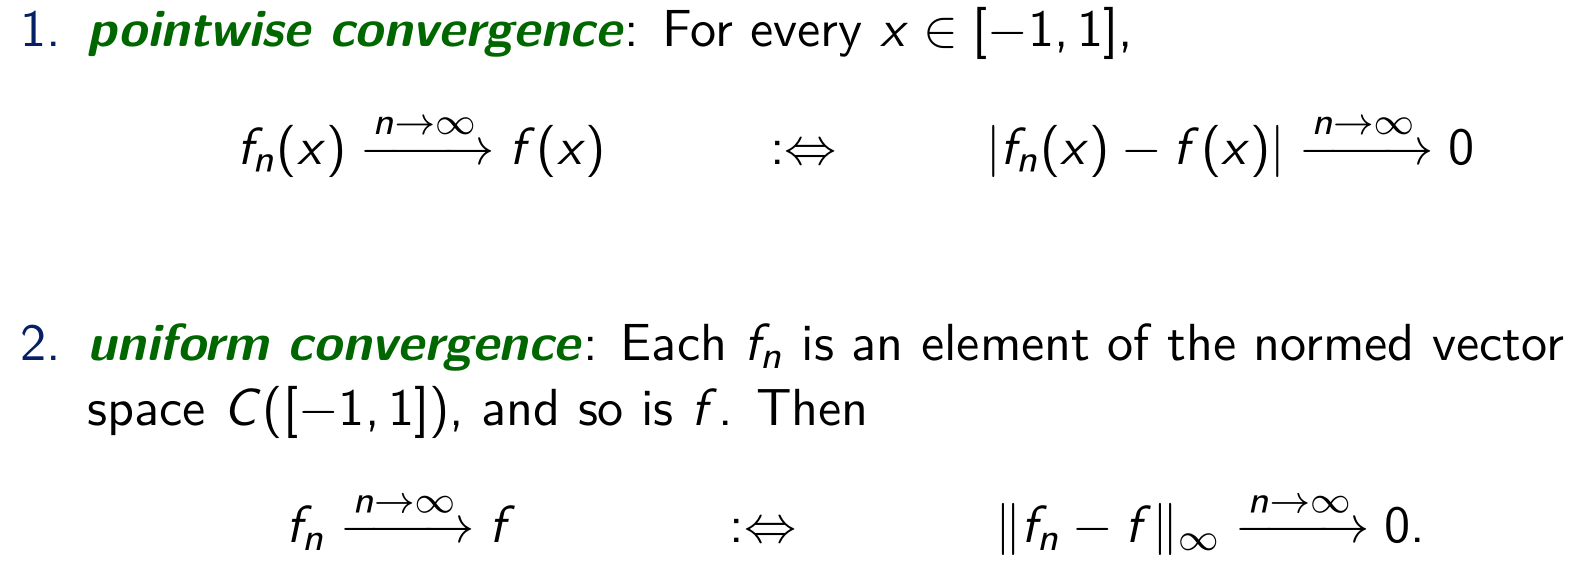
\includegraphics[width=0.9\textwidth]{2020-11-11-12-40-26.png}
    \end{figure}
    \textbf{Remark:}
    \begin{itemize}
        \item 
        Notice that the second definition is more natural in the sense that we consider the convergence of function in a normed vector space of \textbf{functions}. (What is this vector space?)
        \item  What is the difference between the pointwise and uniform convergence of functions ... 
        \item Uniform convergence $\Rightarrow$ pointwise convergence. (Why?) If both limit exist, they coincide with each other.
    \end{itemize} 
\end{frame}

\begin{frame}
    \frametitle{Recall...}

    Describe in words the difference between \textbf{pointwise convergence of function sequence} and \textbf{uniform convergence of function sequence}. How are these two concepts different? If you can, state some properties that they have in common or that serve to differentiate them from each other. Is one of them also always an example of the other? Give examples.
    \nullspace
    This exercise is left for you!
\end{frame}

\begin{frame}
    \frametitle{How to Calculate}

    Here is a common procedure to find the limit of a function sequence $(f_n)$
    \begin{enumerate}
        \item Fix each $x\in\Omega$, find the pointwise limit of $(f_n)$, denoted by $f$.
        \item Fix each $k\in \N$, find an explicit expression of $\|f_k(x)-f(x)\|$, or an estimate of it.
        \item If 2. $\to 0$ as $k\to \infty$, we have $(f_n)$ converges uniformly to $f$. Otherwise, the convergence is pointwise but not uniform.
    \end{enumerate}

\end{frame}
\subsection{Exercise}
\begin{frame}
    \frametitle{Exercise}

    Find the pointwise limit of the sequence of functions $(f_n)$ on $\R$, where
    $$f_n(x)=\dfrac{x^2+nx}{n}.$$ Is this a uniform convergence?

\end{frame}

\begin{frame}
    \frametitle{Completeness of Function Space}

    The metric space $(C([a,b]),\rho)$ is complete, where $\rho(f,g)=\left\|f - g\right\|_\infty$. 

\end{frame}


\begin{frame}
    \frametitle{Uniform Convergence \& Continuity}

    A uniformly convergent sequence of continuous functions will always converge to a continuous function.

    \begin{figure}[H]
        \centering
        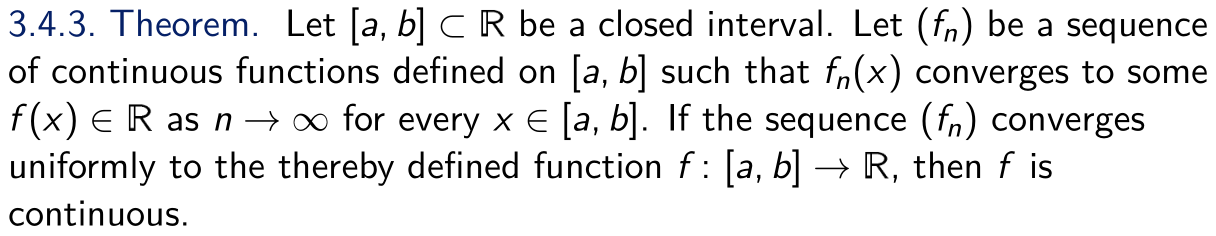
\includegraphics[width=0.9\textwidth]{2020-11-11-12-54-55.png}
    \end{figure}
    
\end{frame}

\section{Series}
\subsection{Definition}
\begin{frame}
    \frametitle{Definition of Series}
    \begin{figure}[H]
        \centering
        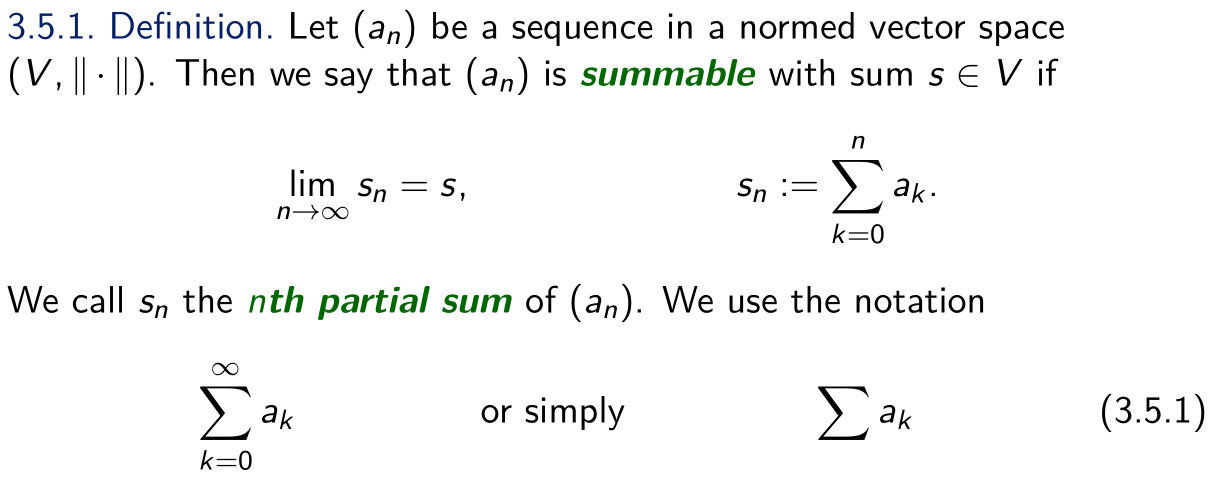
\includegraphics[width=0.9\textwidth]{2020-11-11-12-56-31.png}
    \end{figure}
    \textbf{Remark:} The word ``series'' has two meanings:
    \begin{enumerate}
        \item the limit of $(s_n)$.
        \item the procedure of summing the sequence $(a_n)$.
    \end{enumerate}
    Notice that we define series in general vector space, so it is natural to investigate into a series of matrices and etc. However, we will focus on real sequences and function sequences in VV186.
\end{frame}

\subsection{Terminology}
\begin{frame}
    \frametitle{Terminology}
    For a sequence $(a_n)$ in a normed vector space $(V,\|\cdot\|)$. And define $s_n:=\sum_{k=0}^na_k$. Then the following two arguments are equivalent:
    \begin{enumerate}
        \item The sequence $(a_n)$ is summable.
        \item The sequence $(s_n)$ is convergent.
        \item The series $\sum_{k=0}^\infty a_k$ converges.
    \end{enumerate}
    Think about the difference in description.

\end{frame}

\begin{frame}
    \frametitle{The limit of $(s_n)$}

    It is easier to deduce whether some sequence is summable than finding the concrete sum. This is analogous to finding whether a sequence is convergent. Why? Because a series is the limit of $(s_n)$, a special sequence.
    \nullspace
    For example,
    \begin{itemize}
        \item $(a_n)=\dfrac{1}{n^2}$
        \item $(a_n)=\dfrac{4^n}{n!}$
        \item ...
    \end{itemize}
    \nullspace
    Therefore, we develop several test techniques to help us deduce whether a sequence is summable. Before that, let's discuss the \emph{Cauchy criterion }and \emph{absolute convergence} first, which are fundamental tools in the field of series.
\end{frame}

\subsection{Cauchy Criterion}
\begin{frame}
    \frametitle{Cauchy Criterion}

    \begin{figure}[H]
        \centering
        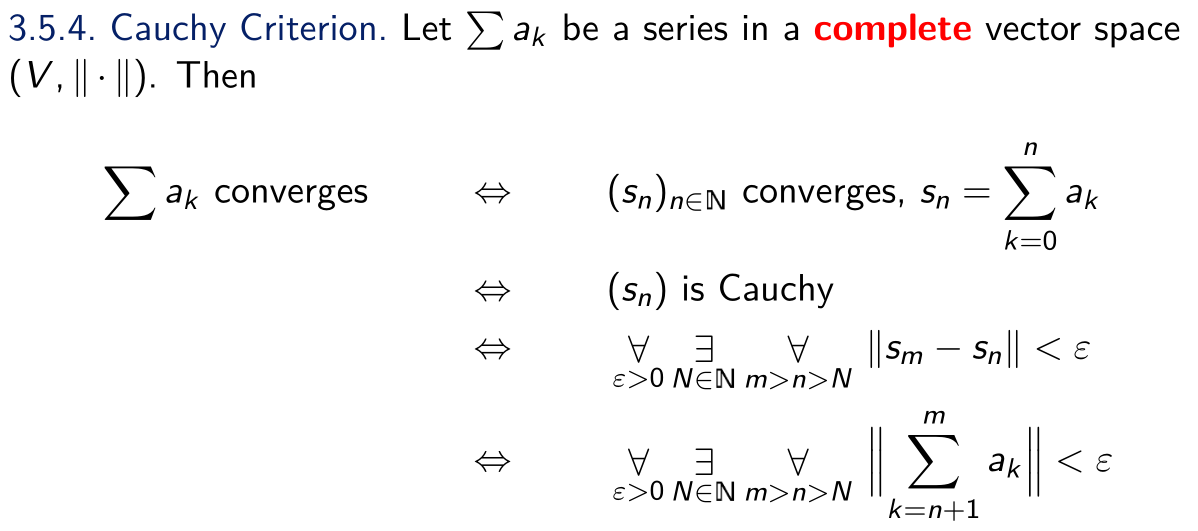
\includegraphics[width=0.9\textwidth]{2020-11-11-13-40-03.png}
    \end{figure}
    \textbf{Remark:} Intuitively speaking, cauchy criterion requires a summable series in a complete space to have a sufficiently ``flat'' tail. It follows several useful corollaries:
    \begin{enumerate}
        \item If summable, $a_k\to 0$ as $k\to \infty$. (Why? What is its contrapositive?)
        \item If summable, $A_n:=\sum_{k=n}^\infty a_k\to 0$ as $n\to \infty$. (Why?) 
    \end{enumerate}
\end{frame}
\subsection{Absolute Convergence}
\begin{frame}
    \frametitle{Absolute Convergence}

    \begin{figure}[H]
        \centering
        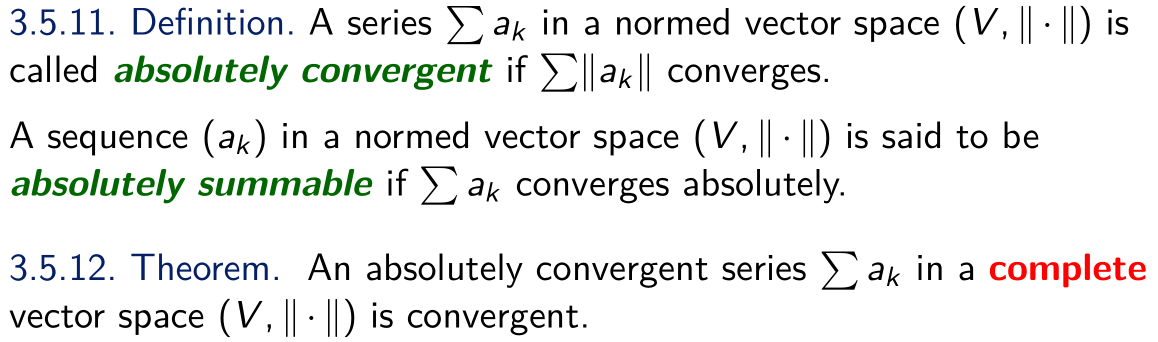
\includegraphics[width=0.9\textwidth]{2020-11-11-13-47-24.png}
    \end{figure}
    \textbf{Remark:} Absolute convergence of series is a strong requirement of summable. We actually do not need absolute convergence to let a sequence summable. If this is the case, we say the series is \emph{conditionally convergent}.\nullspace However, the absolute convergence turns out to be useful because usually a non-negative sequence is easier to deal with.
\end{frame}

\begin{frame}
    \frametitle{Completeness}

    It is worth noting that the previous two theorems (3.5.4 \& 3.5.12) require the vector space $(V,\|\cdot\|)$ to be \alarm{complete}. If you are going to use them in your coursework, the first step is prove the completeness. This is often easy to show but indispensable.

\end{frame}

\begin{frame}
    \frametitle{Infinite Triangle Inequality}

    \begin{figure}[H]
        \centering
        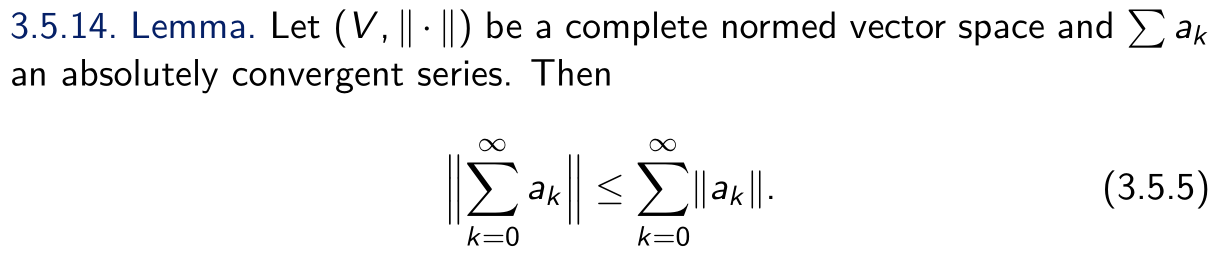
\includegraphics[width=0.9\textwidth]{2020-11-11-14-41-55.png}
    \end{figure}
    
\end{frame}

\begin{frame}
    \frametitle{Proof}

    \begin{figure}[H]
        \centering
        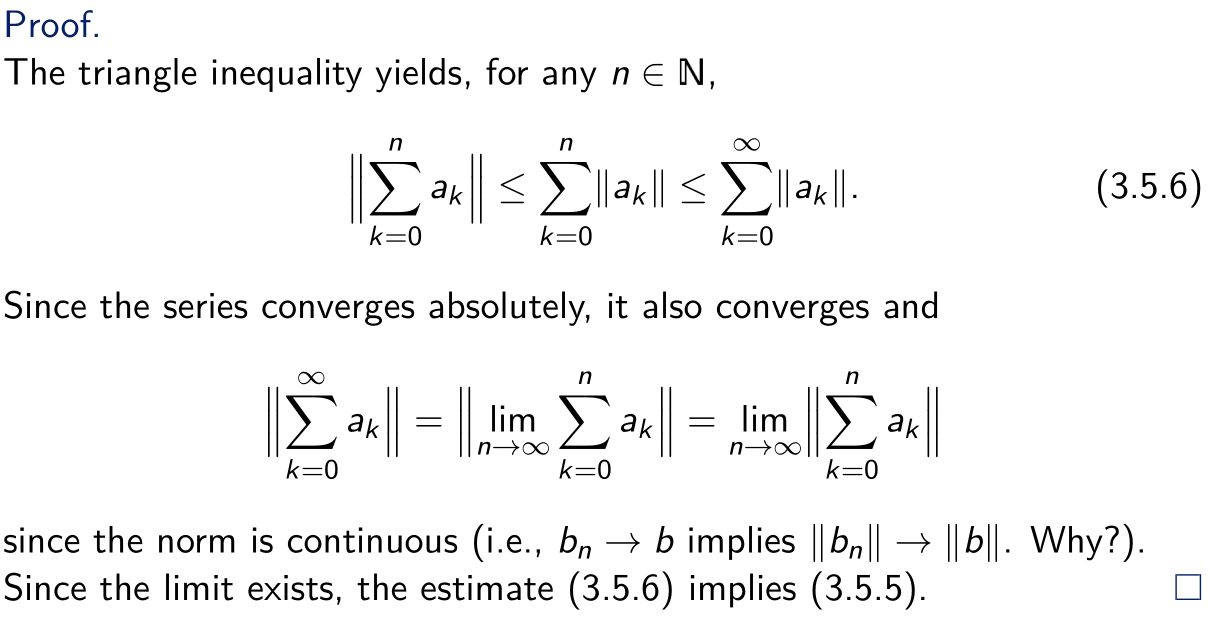
\includegraphics[width=0.9\textwidth]{2020-11-11-14-43-22.png}
    \end{figure}
    Does the last equality trivially hold? No! How can we show that holds given the norm is continous?
\end{frame}

\subsection{Tests of Summable Sequences}
\begin{frame}
    \frametitle{Tests of Summable Sequences}

    For all of the following tests, if the domain of discourse is real sequences, we require the real sequence to be (strictly) positive. Recall that in complete space, absolute convergence implies convergence of series.
    \begin{enumerate}
        \item 3.5.9. Convergence of p-Series
        \item 3.5.15. Comparison test \& Contrapositive
        \item 3.5.19. Weierstra\ss M-test (proof: show pointwise convergence by comparison test, and prove the convergence is uniform)
        \item 3.5.22. Root test (proof: comparison test)
        \item 3.5.26. Root test using limits (proof: root test)
        \item 3.5.28. Ratio test (proof: comparison test)
        \item 3.5.30. Ratio test using limits (proof: similar with 3.5.26)
        \item 3.5.31. Ratio comparison test (proof: comparison test)
        \item 3.5.32. Raabe's test [finer version of ration test] (proof: Bernoulli's inequality \& ration comparison test)
        \item 3.5.38. Leibniz Theorem.
    \end{enumerate}
    \textbf{Remark:} For 4. and 6., we use upper/lower limits in the tests. This can be quite useful when the limit of the target sequence exists. Why?
\end{frame}

\subsection{Exercise}
\begin{frame}
    \frametitle{Exercise - Straightforward}

    Please determine whether the following series converge or not.
    \begin{enumerate}
        \item $\sum\dfrac{4n(n+2)!}{(2n)!}$
        \item $\sum\dfrac{\sin(\alpha n)}{n^2},\quad \alpha\neq 0$
        \item $\sum \dfrac{(2n)!}{4^n(n+1)!n!}$
        \item $\sum \dfrac{1}{(\ln n)^{\ln n}}$
    \end{enumerate}
\end{frame}

\begin{frame}
    \frametitle{Exercise - Abstract}

    Prove that if $(a_n)$ is a non-negative non-summable sequence. Show that
    $$\sum\dfrac{a_n}{1+a_n}$$
    diverges.\footnote[frame]{Spivak \textit{Calculus} p.463}
\end{frame}
\subsection{Cauchy Product \& Convolution}
\begin{frame}
    \frametitle{Cauchy Product \& Convolution}

    \begin{figure}[H]
        \centering
        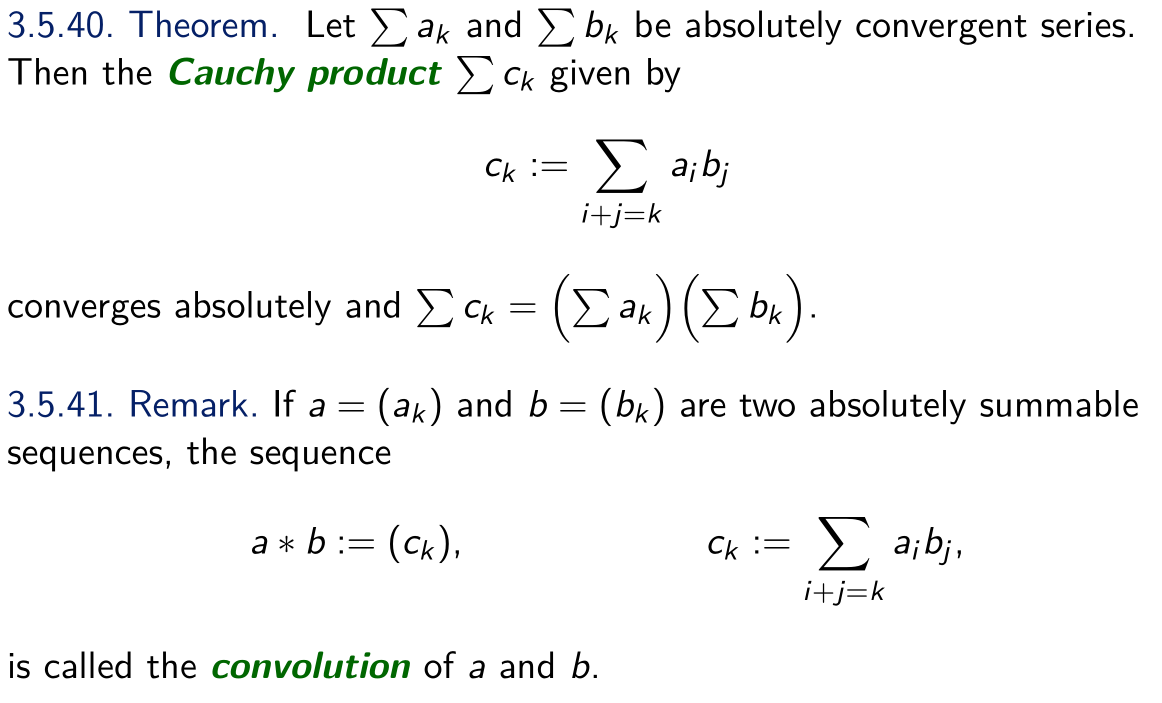
\includegraphics[width=0.9\textwidth]{2020-11-11-15-36-39.png}
    \end{figure}
    \textbf{Remark:} This kind of convolution is called the \emph{discrete} convolution. We will learn \emph{continous} convolution in VV286.

\end{frame}

\section{Extension}
\subsection{Discrete Convolution in Engineering Field}
\begin{frame}[allowframebreaks]
    \frametitle{* Discrete Convolution in Engineering Field}
    \begin{figure}[H]
        \centering
        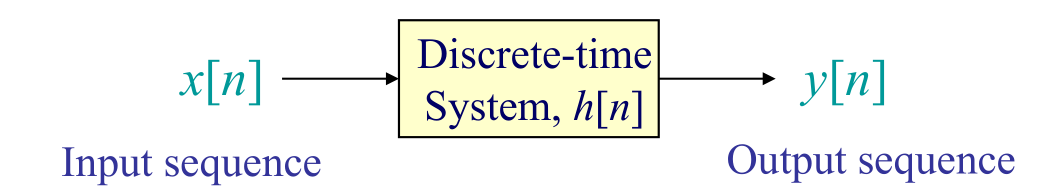
\includegraphics[width=0.6\textwidth]{2020-11-11-16-50-46.png}
        \caption{Discrete Time System}
    \end{figure}
    
    In the field of \emph{Signal Processing}, we can fully characterize a \emph{ discrete linear time-invariant system} using a discrete function (essentially a sequence) $h[n]$, called the \emph{impulse response} of this system. To be more precise, the output signal $y$ and the input signal $x$ has the following relation:
    $$y[n]=h[n]*x[n]$$
    \begin{figure}[H]
        \centering
        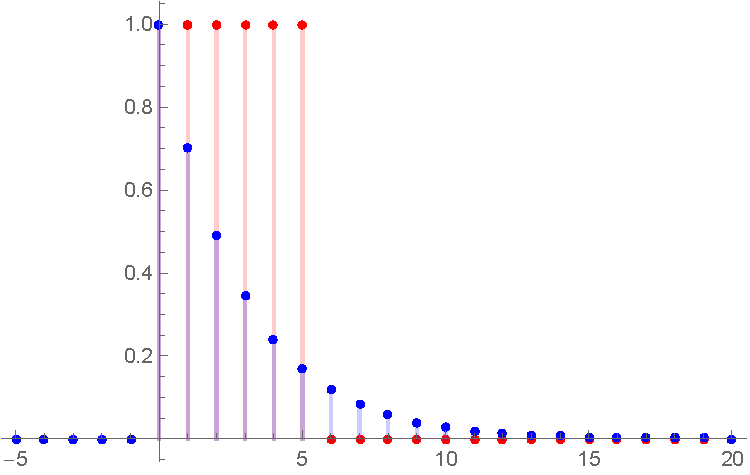
\includegraphics[width=0.5\textwidth]{1.pdf}
        \caption{{\color{red} $h[n]$} and {\color{blue} $x[n]$}}
    \end{figure}
    In this example, our impulse function {\color{red} $h[n]$} is simply a rectangular function. Our input signal {\color{blue} $x[n]$} is a decaying signal. Can you imagine the output signal?

\begin{figure}[H]
    \centering
    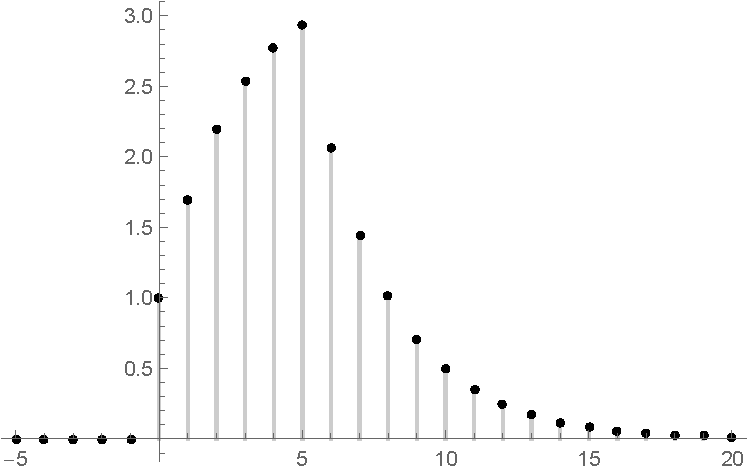
\includegraphics[width=0.5\textwidth]{2.pdf}
    \caption{$y[n]$}
\end{figure}

Think about how the system modifies the input signal. This process will be discussed in detail in \emph{VE216: Signal and System}, a very fundamental engineering discipline.
    
\end{frame}

\begin{frame}
    \frametitle{End}
    \vspace{2.2cm}
    \begin{center}
        \Large
        Have Fun \\
        And \\
        Learn Well!\footnote[frame]{Special acknowledgement to former TA \textbf{Zhang Leyang}, who offered plenty of exercises and advice to my recitation class.}
    \end{center}
\end{frame}

\end{document}